\documentclass[11pt]{article}
\usepackage[margin=1in]{geometry}
\usepackage[T1]{fontenc}
\usepackage[utf8]{inputenc}
\usepackage{lmodern}
\usepackage{microtype}
\usepackage{amsmath,amssymb,mathtools}
\usepackage{booktabs,tabularx,array,longtable}
\usepackage{graphicx}
\usepackage{caption}
\usepackage{xcolor}
\usepackage{enumitem}
\usepackage{hyperref}

\hypersetup{
  colorlinks=true,
  linkcolor=blue,
  citecolor=blue,
  urlcolor=blue
}

\setlength{\parindent}{0pt}
\setlength{\parskip}{0.55em}
\newcolumntype{Y}{>{\raggedright\arraybackslash}X}
\graphicspath{{./}}

\title{\textbf{Integrated Evaluation Report on the Entropy-S EDL Experiments}\\
\large Assessment of the new structural audit in light of the manuscript, codebase, and uploaded results}
\author{Prepared in English from the provided materials}
\date{March 10, 2026}

\begin{document}
\maketitle

\begin{abstract}
This report evaluates the new audit note against three evidence sources: the manuscript draft \texttt{V3.pdf}, the public \texttt{phiark/Entropy-S} repository on branch \texttt{codex/repo-cleanup}, and the uploaded experimental outputs (\texttt{matched\_auroc.csv}, \texttt{risk\_coverage\_summary.csv}, \texttt{matched\_scatter.png}, and \texttt{risk\_coverage\_eta\_0.10.png}). The central conclusion is that the new audit is \emph{substantially correct} and materially deeper than the repair report: the dominant failure is structural, not merely recipe instability. However, the most precise statement is \emph{not} that the KL term and the data-fit term are literally identical. The sharper diagnosis is that the implemented Sensoy-style objective has an unbounded one-hot ray, leaves target evidence scale effectively uncontrolled, and supplies no mechanism that would reliably learn a high-vacuity manifold for truly novel inputs. The ternary $(r,\tau)$ theory in the draft survives; the current EDL instantiation does not realize its intended semantics robustly enough for the benchmark to validate the paper's strongest experimental story.
\end{abstract}

\section{Materials assessed}

This evaluation is based on the following source base:
\begin{itemize}[leftmargin=1.5em]
  \item the manuscript draft \texttt{V3.pdf}, which explicitly positions the work as a modest diagnostic layer rather than a new general uncertainty theory and states that the experiment is meant to test whether residual separation remains after predictive-entropy matching \cite{draft};
  \item the repository README, repair report, training code, utility code, evaluation code, and synthetic demo from \texttt{phiark/Entropy-S} on branch \texttt{codex/repo-cleanup} \cite{readme,repair,train,utils,eval,synthetic};
  \item the uploaded result files \texttt{matched\_auroc.csv} and \texttt{risk\_coverage\_summary.csv}, plus the uploaded figures \texttt{matched\_scatter.png} and \texttt{risk\_coverage\_eta\_0.10.png} \cite{csv-auroc,csv-risk}.
\end{itemize}

I also incorporate the qualitative contrast visible in the four plots shown in the conversation: one regime resembles a high-$r$ fan with weak explicit-unknown semantics, while another resembles a low-$r$ wall with evidence collapse. That two-regime behavior matters, because it suggests that the failure is not a single bug but an instability in how ``unknown'' is realized.

\section{Executive assessment of the new audit note}

\begin{table}[h]
\centering
\small
\caption{Assessment of the major claims in the new audit note}
\begin{tabularx}{\linewidth}{>{\raggedright\arraybackslash}p{0.29\linewidth} >{\raggedright\arraybackslash}p{0.16\linewidth} Y}
\toprule
\textbf{Audit claim} & \textbf{Verdict} & \textbf{Why} \\
\midrule
The failure is structural rather than merely a bad recipe. & Mostly correct & The repair report identifies real hygiene bugs, but the implemented loss geometry still contains an unbounded one-hot direction and does not learn high vacuity for unseen inputs by itself. Tuning learning rate or annealing can change \emph{how fast} this happens, not \emph{what objective is being optimized}. \\
\addlinespace
The KL term and the data-fit term both push evidence toward one-hot, so the problem is intrinsic. & Directionally correct, but imprecise & On non-target classes the two terms are aligned: both suppress evidence. On the target class, however, the KL term is blind rather than aligned. That distinction matters. The structural problem is under-constraint and scale degeneracy, not perfect gradient identity. \\
\addlinespace
The synthetic demo is circular and gives false confidence. & Correct, with a small caveat & The synthetic generator directly writes in the desired high-evidence ID-hard versus low-evidence OOD geometry. It is still a useful sanity check for the \emph{diagnostic chart}, but it is not evidence that the training procedure can realize that chart on real data. \\
\addlinespace
The softplus evidence function creates a nontrivial vacuity floor and explains weak OOD behavior. & Correct and important & This point is stronger than the repair report. At neutral logits, softplus already yields positive evidence, which keeps the model away from the unresolved vertex unless all logits are driven negative together. \\
\bottomrule
\end{tabularx}
\end{table}

In short: the audit note is the better causal account. The repair report is still useful, but mainly as a necessary cleanup of implementation mistakes. It does not reach the deeper reason why the geometry in the paper is hard to realize in the current EDL pipeline.

\section{What the manuscript and the current outputs actually establish}

The manuscript itself is careful about scope. It says the framework is a diagnostic layer for explicit-unknown states, not a replacement for Shannon theory or a new general uncertainty functional \cite{draft}. It also says the CIFAR-10/SVHN experiment is meant to falsify a specific claim: after matching ordinary predictive entropy, does residual separation remain between high-conflict in-distribution samples and low-evidence OOD samples? If not, the framework is ``mostly pedagogical''; if yes, the diagnostic chart is doing real work \cite{draft}.

The uploaded numbers show a \emph{mixed verdict}. On the entropy-matched AUROC task, the pair probe on $(r,H_{\mathrm{cont}})$ reaches about $0.603$, whereas all scalar baselines remain near chance after orientation correction, roughly $0.505$--$0.524$ \cite{csv-auroc}. So the pair does recover some residual structure that predictive entropy does not.

However, on mixed-stream selective risk at $80\%$ coverage, that pair is \emph{worse} than predictive entropy for all tested OOD ratios $\eta \in \{0.1,0.3,0.5\}$ \cite{csv-risk}. This means the pair is useful as a matched diagnostic discriminator, but it is not automatically a good abstention score.

\begin{table}[t]
\centering
\small
\caption{Current uploaded metrics. AUROC is reported with the best monotone orientation for scalar scores, following the repository convention.}
\begin{tabular}{lcccc}
\toprule
\textbf{Score} & \textbf{Matched AUROC} & \textbf{Risk@80\%, $\eta=0.1$} & \textbf{Risk@80\%, $\eta=0.3$} & \textbf{Risk@80\%, $\eta=0.5$} \\
\midrule
Predictive entropy & 0.523 & 0.055 & 0.213 & 0.432 \\
Vacuity & 0.522 & 0.056 & 0.213 & 0.432 \\
Dissonance & 0.505 & 0.097 & 0.276 & 0.475 \\
Resolution ratio $1-r$ & 0.522 & 0.056 & 0.213 & 0.432 \\
Projected entropy $\beta=0.1$ & 0.515 & 0.130 & 0.306 & 0.492 \\
Projected entropy $\beta=0.5$ & 0.523 & 0.055 & 0.214 & 0.433 \\
Projected entropy $\beta=0.75$ & 0.524 & 0.056 & 0.217 & 0.436 \\
Pair probe $(r,H_{\mathrm{cont}})$ & 0.603 & 0.105 & 0.257 & 0.449 \\
\\
\bottomrule
\end{tabular}
\end{table}

This table already hints at the correct synthesis:

\begin{enumerate}[leftmargin=1.5em]
  \item The diagnostic plane is \emph{not empty}. There is some residual signal.
  \item But the signal is weaker and more task-specific than the draft's strongest experimental narrative hoped for.
  \item Therefore the main question becomes: \emph{why does the model fail to realize the intended explicit-unknown semantics robustly?}
\end{enumerate}

\section{Structural analysis of the implemented EDL loss}

The repository implements a Sensoy-style evidential classification loss of the form
\begin{align}
\alpha_k &= \operatorname{softplus}(z_k) + 1, \\
S &= \sum_{j=1}^K \alpha_j, \qquad p_k = \frac{\alpha_k}{S}, \\
\mathcal{L}_{\mathrm{EDL}} &= \sum_{k=1}^K \left[(y_k-p_k)^2 + \frac{\alpha_k(S-\alpha_k)}{S^2(S+1)}\right]
+ \lambda_t \, \mathrm{KL}\!\left(\mathrm{Dir}(\tilde{\alpha}) \,\|\, \mathrm{Dir}(\mathbf{1})\right),
\end{align}
where $\tilde{\alpha}_y=1$ and $\tilde{\alpha}_{j\neq y}=\alpha_j$, and the KL weight is annealed in training \cite{utils,train}.

The repair report interprets the bad behavior of pure EDL mainly as recipe instability: augmentation sensitivity, fast annealing, and an aggressive learning rate. That explanation is incomplete. The more important point is structural:

\subsection*{A zero-loss ray exists}

Fix a training example with class label $y$. Consider the ray
\[
\alpha_y = a, \qquad \alpha_j = 1 \quad (j\neq y), \qquad a\ge 1.
\]
Along this ray, the KL term vanishes \emph{exactly}, because $\tilde{\alpha}=\mathbf{1}$. Meanwhile the data-fit term becomes
\[
\mathcal{L}_{\mathrm{data}}(a)
= \frac{K^2+K-2}{a^2 + (2K-1)a + K(K-1)}
\;\longrightarrow\; 0
\qquad \text{as } a\to\infty.
\]

For the actual case $K=10$, this reduces to
\[
\mathcal{L}_{\mathrm{data}}(a) = \frac{108}{a^2 + 19a + 90} \to 0.
\]

This is the key structural fact. The implemented loss has an infimum at an arbitrarily sharp one-vs-all state with unbounded target evidence and zero non-target evidence. Lower learning rate, longer annealing, or temporary backbone freezing may make optimization \emph{less violent}, but they do not remove this ray.

\subsection*{What the audit note gets right -- and what should be phrased more carefully}

The new audit says that the data-fit and KL terms are ``homomorphic'' in optimization direction and both push evidence toward one-hot. That statement is directionally right on the non-target coordinates: both terms discourage evidence on wrong classes. But it is not literally right on the target coordinate. The target coordinate is not regularized upward by the KL term; it is effectively \emph{left unregularized}. The more precise diagnosis is:

\begin{quote}
The implemented objective is under-constrained. It suppresses non-target evidence, leaves target evidence scale essentially free, and therefore admits an unbounded one-hot ray.
\end{quote}

That refinement matters because it points to the right remedy. The remedy is not just gentler optimization. It is either (i) a different evidential objective, or (ii) an explicit additional mechanism that constrains evidence scale and teaches when \emph{not} to commit evidence.

\section{Why OOD vacuity is structurally difficult under softplus evidence}

The audit note's point about the evidence function is excellent and should be retained.

If all logits are neutral, $z_k=0$ for every class, then
\[
e_k = \operatorname{softplus}(0)=\log 2 \approx 0.693,
\qquad
\alpha_k = 1+\log 2.
\]
Therefore
\[
u = \frac{K}{\sum_j \alpha_j}
= \frac{K}{K(1+\log 2)}
= \frac{1}{1+\log 2}
\approx 0.5906,
\]
and
\[
r = 1-u = \frac{\log 2}{1+\log 2} \approx 0.4094.
\]

Two consequences follow immediately.

First, even a completely neutral logit vector does \emph{not} lie near the unresolved vertex. The parameterization itself places the model at moderate commitment by default.

Second, to obtain genuinely high vacuity, every logit must be pushed deep into the negative regime \emph{simultaneously}. Under equal logits, to achieve $u\ge 0.95$ one needs
\[
\operatorname{softplus}(z)\le 0.0526
\quad\Longrightarrow\quad
z \lesssim -2.92.
\]
To achieve $u\ge 0.99$, one needs $z\lesssim -4.59$.

The repository does not provide any training signal that explicitly teaches this behavior on novel inputs. The model is trained on one-hot CIFAR-10 labels only, and the evaluation then asks whether SVHN will land in a low-evidence region \cite{train,eval}. That is a strong hope, not something the current loss identifies. So the weak or unstable vacuity behavior on OOD data is not surprising.

This is why the audit note is right to insist that the problem is deeper than recipe stability. The current model is not merely hard to optimize; it is poorly specified for the semantic job the paper wants it to do.

\section{Why the synthetic demo succeeds too easily}

The synthetic demo samples ID-hard and OOD cohorts with explicitly different evidence geometry. The ID-hard generator uses substantially higher total evidence and two competing top classes, while the OOD generator uses lower total evidence plus one more dominant pseudo-class \cite{synthetic}. In other words, the generator assumes exactly the pattern the real experiment is supposed to discover.

That is why the synthetic demo looks so clean. It is a conditional validation of the following implication:

\begin{quote}
\emph{If} the model produces high-evidence conflict for ID-hard points and low-evidence diffuse commitment for OOD points, \emph{then} the $(r,H_{\mathrm{cont}})$ chart makes the distinction visible.
\end{quote}

That implication is useful. It validates the chart, not the learner.

So the audit note is right to call attention to the circularity. I would phrase it slightly more mildly than ``the validation is meaningless,'' because the demo still works as a sanity check of the \emph{diagnostic reduction}. But it absolutely cannot be used as evidence that the actual EDL training recipe is close to solving the real problem.

\section{Important issues the audit note does not fully cover}

The new audit is good, but the full diagnosis is even broader. Several additional issues appear in the manuscript-code-results triangle.

\subsection{The benchmark cohort is model-dependent}

The evaluation script defines the CIFAR-10 ID-hard subset by the smallest top-2 probability margins of the \emph{same model being evaluated} \cite{eval,draft}. If a model collapses to low evidence or near-uniform predictions, that very collapse can create small margins and cause those points to be selected as ``hard ID''. This contaminates the benchmark. It means the cohort is not fixed across CE, EDL, and warm-started EDL.

As a result, a CE checkpoint and an EDL checkpoint are not being compared on the same hard-ID set. That weakens any conclusion about which geometry is better.

\subsection{Raw $H_{\mathrm{cont}}$ is used even where the paper's own geometry says it is unreliable}

The manuscript's Fisher metric makes the content direction carry weight proportional to $r$ and explicitly notes that the content fiber collapses as $r\to 0$ \cite{draft}. Yet the current evaluation uses raw $H_{\mathrm{cont}}=h(\tau)$ as a full-strength feature in the pair probe even in the low-$r$ regime \cite{utils,eval}.

That is theoretically inconsistent with the draft's own geometry. In the current uploaded scatter, many points form a dense wall near $r\approx 0$, where $H_{\mathrm{cont}}$ should be treated with caution rather than as an equally reliable coordinate. A more faithful evaluation would either threshold on $r$ or use $r\,H_{\mathrm{cont}}$ rather than raw $H_{\mathrm{cont}}$.

\subsection{The pair probe is trained for one task and reused for another}

The pair probe is trained on entropy-matched OOD-versus-ID-hard discrimination and then reused as an abstention score on the mixed CIFAR-10/SVHN selective-risk task \cite{eval}. Those are not the same decision problem. The numbers make this mismatch visible: the pair helps on the matched AUROC task, but it hurts on mixed-stream selective risk \cite{csv-auroc,csv-risk}.

So part of the negative result is not ``the pair has no information.'' It is ``the same learned decision surface is being used for a different utility.''

\subsection{CE checkpoints are pseudo-evidentialized rather than genuinely explicit-unknown}

The evaluation code always converts logits to evidential parameters via
\[
\alpha = \operatorname{softplus}(z)+1
\]
before computing vacuity, $r$, $\tau$, and $H_{\mathrm{cont}}$ \cite{eval}. For an EDL model that is natural. For a pure CE model, it is only a post hoc reinterpretation. So a CE-versus-EDL comparison on evidential coordinates is partly apples versus post-processed oranges.

This matters because one of the plot regimes shown in the conversation looks exactly like such a pseudo-evidential CE geometry: high-$r$, fan-shaped, and only weakly using the unknown axis.

\subsection{Some baselines are duplicates by construction}

In the current implementation, vacuity is exactly $p_u$, while the ``resolution ratio'' abstention score is implemented as $1-r$, which is the same quantity \cite{readme,utils,eval}. That is why the two columns in the risk table are numerically identical. This is not a fatal issue, but it means the baseline set is smaller than it may appear.

\section{Theory, model, and benchmark: where the failure actually sits}

The cleanest integrated diagnosis is a three-level one.

\subsection*{Theory level: mostly intact}

The manuscript's mathematical claims are modest and remain intact as mathematics. The decomposition
\[
H_3(\sigma)=h(r)+r h(\tau)
\]
is just a chain-rule identity, the completion map is non-injective, and the decision-blindness theorem is conceptually sound \cite{draft}. The current experiments do not refute those claims.

Indeed, one negative empirical result is actually \emph{consistent} with the theory: the paper predicts that no single completion parameter $\beta$ should remove decision blindness uniformly, and the uploaded results show that $\beta=0.1$ performs especially badly on the mixed-risk task \cite{draft,csv-risk}.

\subsection*{Model-instantiation level: this is where the main failure lies}

The current EDL pipeline does not identify the semantic unknown state that the paper wants. The reasons are structural:

\begin{itemize}[leftmargin=1.5em]
  \item one-hot ID supervision does not teach a distinction between ambiguity and novelty;
  \item the implemented EDL objective has an unbounded one-hot ray;
  \item softplus evidence creates a neutral vacuity floor far from the unresolved vertex;
  \item there is no explicit OOD or abstention signal telling the network when to keep total evidence low.
\end{itemize}

This is the core of the problem.

\subsection*{Benchmark-design level: also problematic}

The evaluation is additionally weakened by moving cohorts, low-$r$ misuse of raw $H_{\mathrm{cont}}$, and task mismatch between matched discrimination and selective abstention. These do not create the entire failure, but they make the conclusions noisier than they need to be.

\section{Can the project continue? Yes, but only with a pivot}

The project is still viable, but the claim must change. The right continuation is \emph{not} ``with enough tuning, EDL will probably show the ideal geometry.'' The right continuation is:

\begin{quote}
The ternary diagnostic theory may be valid, but standard EDL does not stably instantiate the required explicit-unknown semantics on CIFAR-10/SVHN without stronger modeling assumptions.
\end{quote}

A realistic next-stage program would be:

\begin{enumerate}[leftmargin=1.5em]
  \item \textbf{Freeze the evaluation cohort.} Define hard-ID and matched subsets once using a strong reference model, and reuse them for every compared checkpoint.
  \item \textbf{Respect the low-$r$ geometry.} Replace raw $H_{\mathrm{cont}}$ by $rH_{\mathrm{cont}}$, or ignore content statistics below an $r$ threshold.
  \item \textbf{Test whether the evidence function is the bottleneck.} Compare softplus, shifted-softplus, and ReLU-style evidence maps. The neutral-point vacuity floor should be explicitly reported.
  \item \textbf{Add an explicit unknown signal.} Use outlier exposure, noise or texture OE, or a dedicated abstention objective so the model is actually taught to reduce total evidence on non-ID inputs.
  \item \textbf{Decouple resolution from content in the architecture.} If the paper's object of interest is $(r,\tau)$, a model with a dedicated resolution gate and a separate conditional content head is more faithful than hoping both coordinates emerge from one Dirichlet evidence vector.
  \item \textbf{Separate tasks in reporting.} Keep entropy-matched OOD-versus-ID-hard discrimination and mixed-stream selective rejection as two distinct evaluation problems.
\end{enumerate}

If these steps still fail, the paper can still become a strong \emph{conditional or negative-result paper}: the theory is useful as a diagnostic language, but standard EDL is not the right vehicle for realizing it.

\section{Final verdict}

The new audit note is, overall, the more convincing report.

It is correct that the repair report's ``recipe instability'' diagnosis is too shallow. The main issue is structural: the implemented EDL objective and evidence parameterization do not naturally learn the explicit-unknown state that the paper's benchmark presupposes.

But the audit note should be sharpened in one place. The crucial failure is not that the KL term and the data-fit term are perfectly identical in direction. It is that the loss suppresses non-target evidence, fails to regularize target evidence scale, and never teaches the network when to stay near the unresolved vertex on truly novel inputs. That is why tuning may soften the pathology but cannot solve it.

So the best integrated conclusion is:

\begin{enumerate}[leftmargin=1.5em]
  \item \textbf{The theory is not the main thing that broke.}
  \item \textbf{The current EDL model is the main thing that broke.}
  \item \textbf{The current benchmark design also adds avoidable noise.}
  \item \textbf{The project can continue, but only if it pivots from ``EDL validates the theory'' to ``the theory is sound, but its standard EDL instantiation is structurally inadequate and must be redesigned or carefully delimited.''}
\end{enumerate}

\begin{figure}[p]
\centering
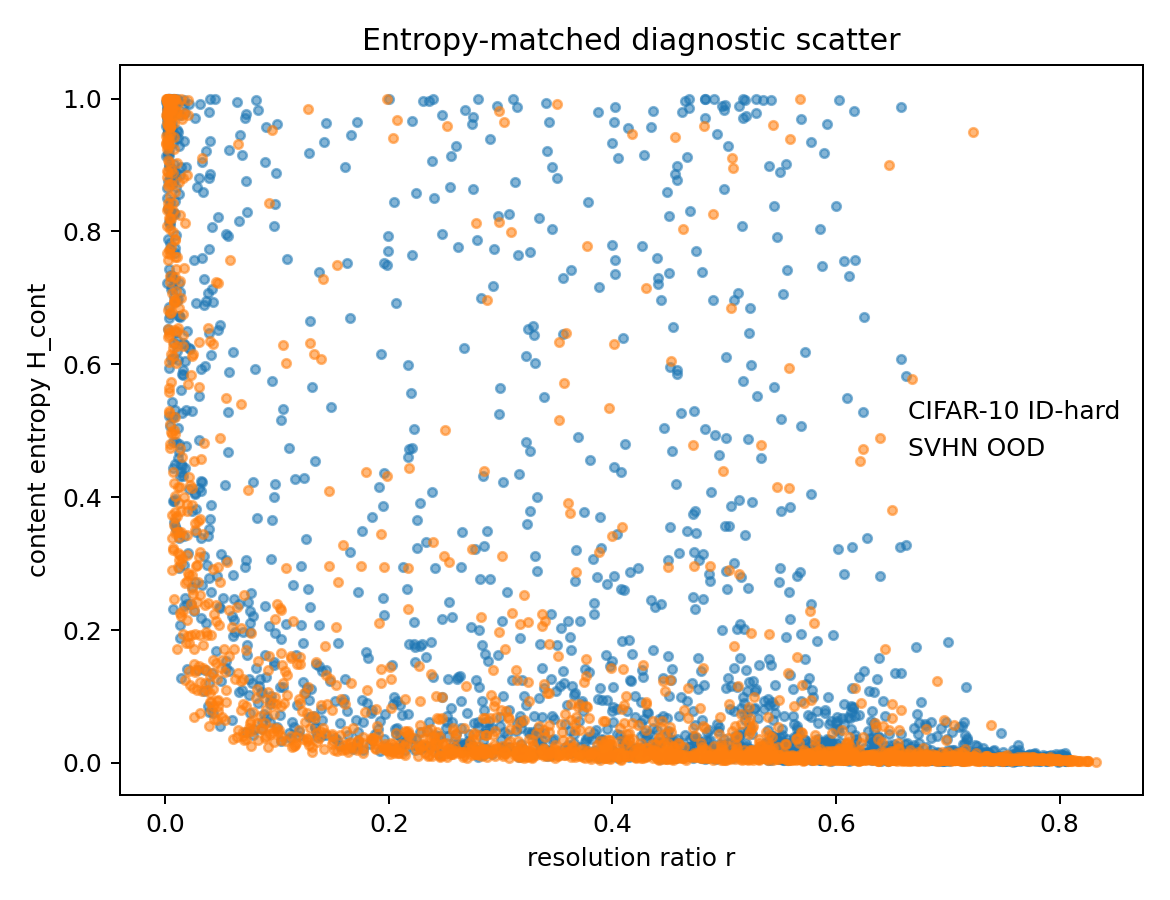
\includegraphics[width=0.88\linewidth]{matched_scatter.png}
\caption{Uploaded entropy-matched scatter. The current regime is not the ideal clean separation described in the draft. OOD points do show a low-$r$ wall, but the ID-hard cohort also spreads deeply into low-$r$ territory, indicating cohort contamination, low-evidence collapse, or both.}
\label{fig:scatter}
\end{figure}

\begin{figure}[p]
\centering
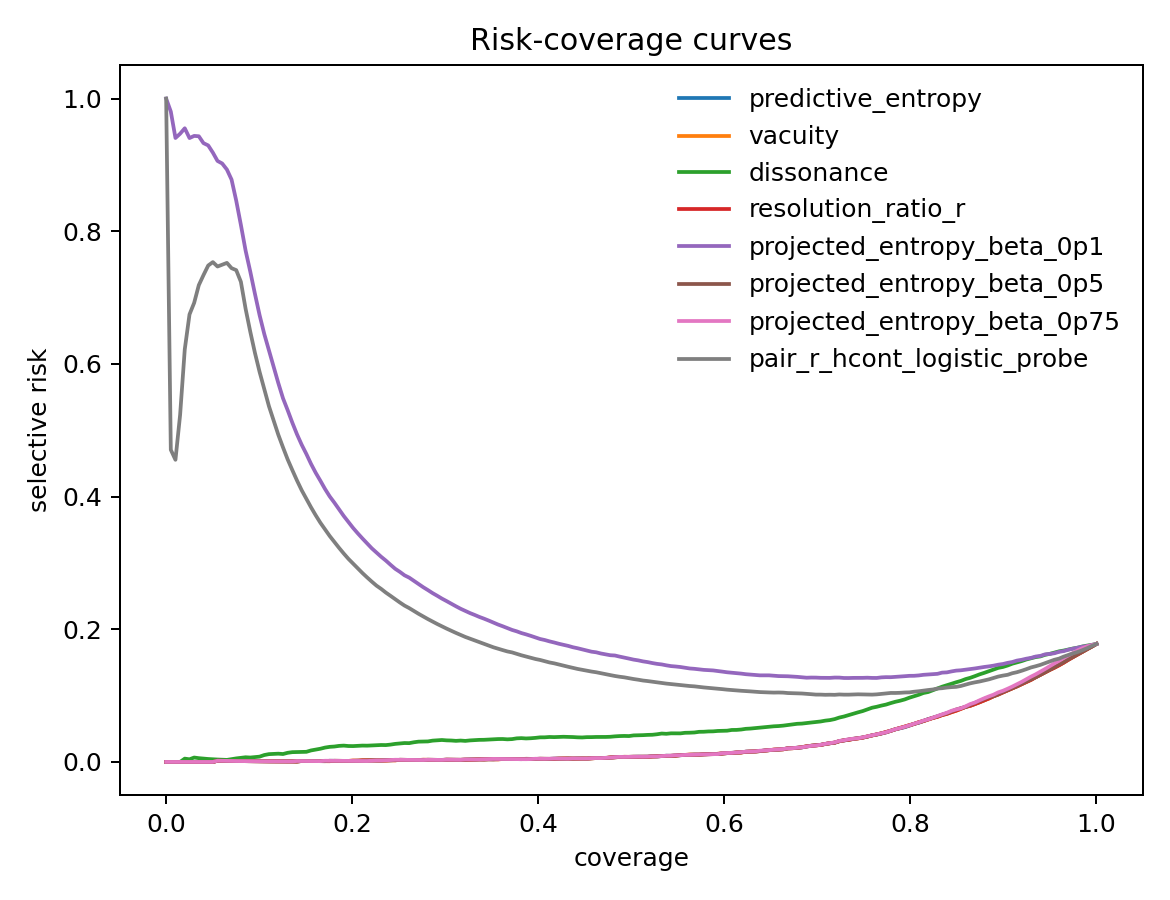
\includegraphics[width=0.88\linewidth]{risk_coverage_eta_0.10.png}
\caption{Uploaded risk-coverage curve for $\eta=0.10$. The pair probe and $\beta=0.1$ projected entropy underperform the simpler uncertainty scores on the selective-risk objective, even though the pair helps on the matched AUROC task.}
\label{fig:risk}
\end{figure}

\begin{thebibliography}{99}

\bibitem{draft}
Rui Li.
\newblock \emph{Resolution-aware Uncertainty Diagnostics for Explicit-Unknown States:
Ternary Coordinates, Projection Loss, and Information Measures}.
\newblock Uploaded manuscript draft \texttt{V3.pdf}, March 2026.

\bibitem{readme}
\texttt{phiark/Entropy-S}, README on branch \texttt{codex/repo-cleanup}.
\newblock \url{https://github.com/phiark/Entropy-S}
\newblock Accessed March 10, 2026.

\bibitem{repair}
\texttt{phiark/Entropy-S}, \texttt{REPAIR\_REPORT.md}.
\newblock \url{https://github.com/phiark/Entropy-S/blob/codex/repo-cleanup/REPAIR_REPORT.md}
\newblock Accessed March 10, 2026.

\bibitem{train}
\texttt{phiark/Entropy-S}, \texttt{train\_edl\_cifar10.py}.
\newblock \url{https://github.com/phiark/Entropy-S/blob/codex/repo-cleanup/train_edl_cifar10.py}
\newblock Accessed March 10, 2026.

\bibitem{utils}
\texttt{phiark/Entropy-S}, \texttt{utils\_evidential.py}.
\newblock \url{https://github.com/phiark/Entropy-S/blob/codex/repo-cleanup/utils_evidential.py}
\newblock Accessed March 10, 2026.

\bibitem{eval}
\texttt{phiark/Entropy-S}, \texttt{evaluate\_resolution\_diagnostics.py}.
\newblock \url{https://github.com/phiark/Entropy-S/blob/codex/repo-cleanup/evaluate_resolution_diagnostics.py}
\newblock Accessed March 10, 2026.

\bibitem{synthetic}
\texttt{phiark/Entropy-S}, \texttt{synthetic\_resolution\_demo.py}.
\newblock \url{https://github.com/phiark/Entropy-S/blob/codex/repo-cleanup/synthetic_resolution_demo.py}
\newblock Accessed March 10, 2026.

\bibitem{csv-auroc}
Uploaded result file \texttt{matched\_auroc.csv}.

\bibitem{csv-risk}
Uploaded result file \texttt{risk\_coverage\_summary.csv}.

\end{thebibliography}

\end{document}
